\documentclass{alex_hü}

\name{Alexander Helbok}
\course{PS Physik}
\hwnumber{11}

\usetikzlibrary{decorations.pathmorphing}
\pgfdeclaredecoration{Snake}{initial}
{
	\state{initial}[switch if less than=+.625\pgfdecorationsegmentlength to final,
	width=+.3125\pgfdecorationsegmentlength,
	next state=down]{
		\pgfpathmoveto{\pgfqpoint{0pt}{\pgfdecorationsegmentamplitude}}
	}
	\state{down}[switch if less than=+.8125\pgfdecorationsegmentlength to end down,
	width=+.5\pgfdecorationsegmentlength,
	next state=up]{
		\pgfpathcosine{\pgfqpoint{.25\pgfdecorationsegmentlength}{-1\pgfdecorationsegmentamplitude}}
		\pgfpathsine{\pgfqpoint{.25\pgfdecorationsegmentlength}{-1\pgfdecorationsegmentamplitude}}
	}
	\state{up}[switch if less than=+.8125\pgfdecorationsegmentlength to end up,
	width=+.5\pgfdecorationsegmentlength,
	next state=down]{
		\pgfpathcosine{\pgfqpoint{.25\pgfdecorationsegmentlength}{\pgfdecorationsegmentamplitude}}
		\pgfpathsine{\pgfqpoint{.25\pgfdecorationsegmentlength}{\pgfdecorationsegmentamplitude}}
	}
	\state{end down}[width=+.3125\pgfdecorationsegmentlength,
	next state=final]{
		\pgfpathcosine{\pgfqpoint{.15625\pgfdecorationsegmentlength}{-.5\pgfdecorationsegmentamplitude}}
		\pgfpathsine{\pgfqpoint{.15625\pgfdecorationsegmentlength}{-.5\pgfdecorationsegmentamplitude}}
	}
	\state{end up}[width=+.3125\pgfdecorationsegmentlength,
	next state=final]{
		\pgfpathcosine{\pgfqpoint{.15625\pgfdecorationsegmentlength}{.5\pgfdecorationsegmentamplitude}}
		\pgfpathsine{\pgfqpoint{.15625\pgfdecorationsegmentlength}{.5\pgfdecorationsegmentamplitude}}
	}
	\state{final}{\pgfpathlineto{\pgfpointdecoratedpathlast}}
}

\begin{document}
\renewcommand{\labelenumi}{\alph{enumi})}


\begin{mybox}{Diamantstruktur}
	\centering \(  \)
	\tcblower
	\begin{enumerate}
		\item \(  \)
%		\begin{flalign*}
%			
%		\end{flalign*}
	\tcbline
		\item \(  \)
%		\begin{flalign*}
%		
%		\end{flalign*}
	\tcbline
		\item \(  \)
%		\begin{flalign*}
%			
%		\end{flalign*}
	\end{enumerate}
\end{mybox}

\begin{mybox}{Gitter, Kristallstruktur und Röntgenbeugung}
	\centering \( \vec{a}_1 = 2a\vec{e}_x;\quad \vec{a}_2 = a(\vec{e}_x + \vec{e}_y);\quad \vec{a}_3 = a\vec{e}_z;\quad \vec{r}_{\text{A}} = 0;\quad \vec{r}_{\text{B}}	 = \vec{a}_1/2 \)
	\tcblower
	\begin{enumerate}
		\item \(  \)
		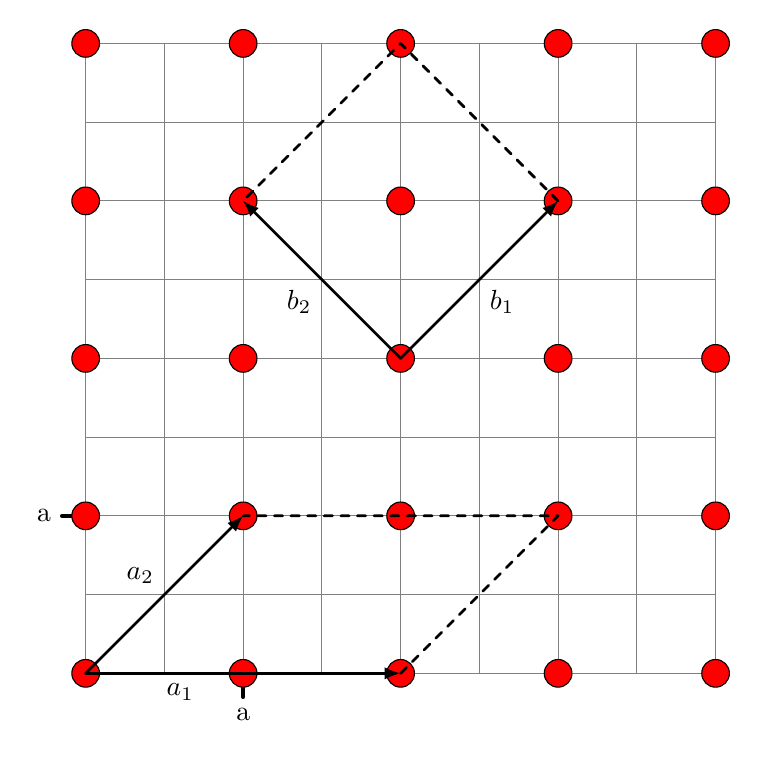
\begin{tikzpicture}[line cap=round,line join=round]
			\draw [color=gray, xstep=1cm,ystep=1cm] (0, 0) grid (8,8);
			
			\draw [line width=1.5pt] (2,-0.3) -- (2, 0.1) node [below, pos=0] {a};
			\draw [line width=1.5pt] (-0.3, 2) -- (0.1, 2) node [left, pos=0] {a};
			
%			\draw[fill=red] (0,0) circle (5pt);
			\begin{scope}
				\clip (-0.2,-0.2) rectangle (8.2, 8.2);
				\foreach \i in {0, 1, 2}{
					\foreach \j in {0, 2, 4}{
					\draw[fill=red] (4*\i,2*\j) circle (5pt);
					\draw[fill=red] (2+4*\i,2*\j) circle (5pt);}}
				
				\foreach \i in {0, 1, 2}{
					\foreach \j in {1, 3}{
						\draw[fill=red] (2+4*\i,2*\j) circle (5pt);
						\draw[fill=red] (4*\i,2*\j) circle (5pt);}}
			\end{scope}
			\draw[-latex, line width=1pt] (0,0) -- (4,0) node [below, pos=0.3] {\( \oldvec{a}_1 \)};
			\draw[-latex, line width=1pt] (0,0) -- (2,2) node [above left, pos=0.5] {\( \oldvec{a}_2 \)};
			\draw[dashed, line width=1pt] (4,0) -- (6,2) -- (2,2);
			
			\draw[-latex, line width=1pt] (4,4) -- (6,6) node [below right, pos=0.5] {\( \oldvec{b}_1 \)};
			\draw[-latex, line width=1pt] (4,4) -- (2,6) node [below left, pos=0.5] {\( \oldvec{b}_2 \)};
			\draw[dashed, line width=1pt] (6,6) -- (4,8) -- (2,6);
		\end{tikzpicture}\\
		The unit cell is not primitive, as it contains more than one lattice point
	\tcbline
		\item \(  \)
		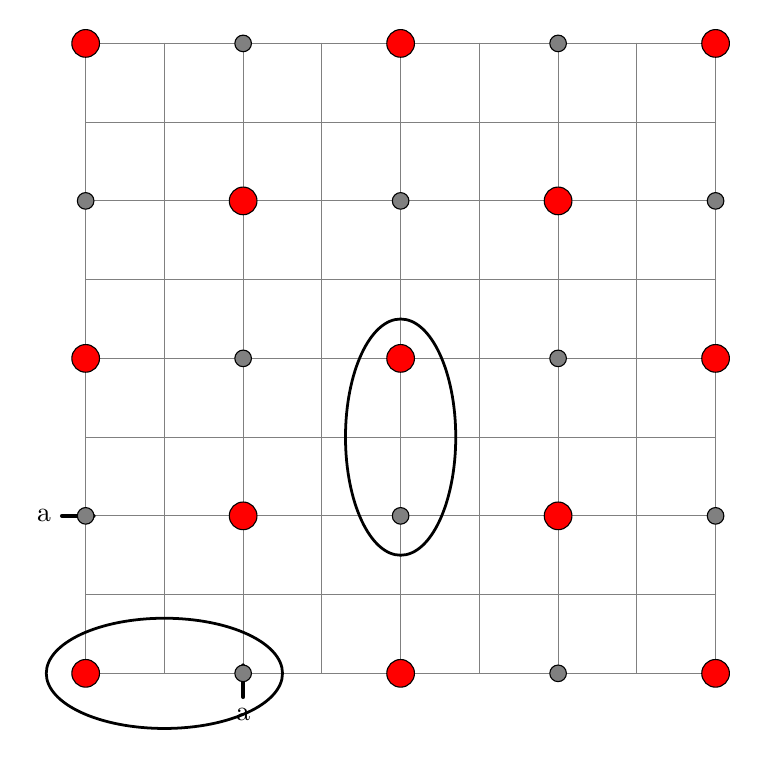
\begin{tikzpicture}[line cap=round,line join=round]
			\draw [color=gray, xstep=1cm,ystep=1cm] (0, 0) grid (8,8);
			
			\draw [line width=1.5pt] (2,-0.3) -- (2, 0.1) node [below, pos=0] {a};
			\draw [line width=1.5pt] (-0.3, 2) -- (0.1, 2) node [left, pos=0] {a};
			
			\begin{scope}
				\clip (-0.2,-0.2) rectangle (8.2, 8.2);
				\foreach \i in {0, 1, 2}{
					\foreach \j in {0, 2, 4}{
						\draw[fill=red] (4*\i,2*\j) circle (5pt);
						\draw[fill=gray] (2+4*\i,2*\j) circle (3pt);}}
				
				\foreach \i in {0, 1, 2}{
					\foreach \j in {1, 3}{
						\draw[fill=red] (2+4*\i,2*\j) circle (5pt);
						\draw[fill=gray] (4*\i,2*\j) circle (3pt);}}
			\end{scope}
			\draw [line width=1pt] (1,0) ellipse (1.5cm and 0.7cm);
			\draw [line width=1pt] (4,3) ellipse (0.7cm and 1.5cm);
		\end{tikzpicture}\\
	\tcbline
		\item \(  \)
		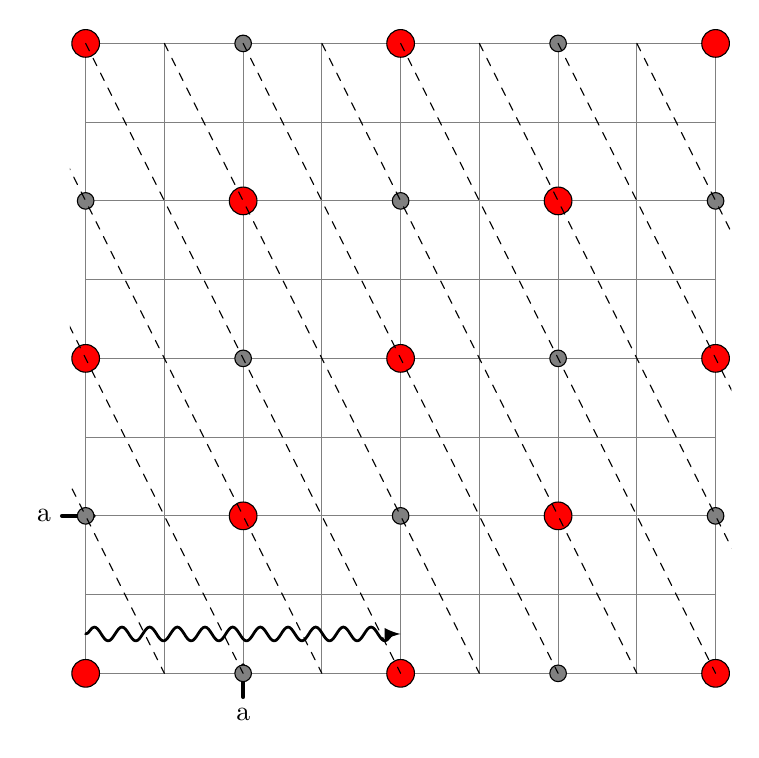
\begin{tikzpicture}[line cap=round,line join=round]
			\draw [color=gray, xstep=1cm,ystep=1cm] (0, 0) grid (8,8);
			
			\draw [line width=1.5pt] (2,-0.3) -- (2, 0.1) node [below, pos=0] {a};
			\draw [line width=1.5pt] (-0.3, 2) -- (0.1, 2) node [left, pos=0] {a};
			
			\begin{scope}
				\clip (-0.2,-0.2) rectangle (8.2, 8.2);
				\foreach \i in {0, 1, 2}{
					\foreach \j in {0, 2, 4}{
						\draw[fill=red] (4*\i,2*\j) circle (5pt);
						\draw[fill=gray] (2+4*\i,2*\j) circle (3pt);}}
				
				\foreach \i in {0, 1, 2}{
					\foreach \j in {1, 3}{
						\draw[fill=red] (2+4*\i,2*\j) circle (5pt);
						\draw[fill=gray] (4*\i,2*\j) circle (3pt);}}
				\foreach \i in {1,...,11}{
					\draw[dashed] (-4+\i, 8) -- (0+\i,0);}
			\end{scope}
			\draw[-latex, line width=1pt, decoration={snake}, decorate] (0, 5mm) -- ++(4,0);
%			\draw[line width=1pt, snake=coil, segment aspect=0, shorten >= 50pt] (1in,2in) -- ++(0.375in,-0.75in);
		\end{tikzpicture}\\
		The X-Ray gets reflected by the crystal and leaves in the negative x-Direction
		\item \( \lambda = 1.46 \unit{\angstrom};\quad \theta = \ang{15} \)
			\begin{flalign*}
				2a\sin(\theta) &= n\lambda &&\\
				a &= \tfrac{\lambda}{2\sin(\theta)} = \dl{2.82 \unit{\angstrom}} &&
			\end{flalign*}
		\item \( \left\{h, k, l\right\} = (2 1 0);\quad \left\{u_1, v_1, w_1\right\} = (0, 0, 0);\quad \left\{u_2, v_2, w_2\right\} = (0.5, 0, 0) \)
			\begin{flalign*}
				F_{210} &= f_{\text{A}} + f_{\text{B}} \expo[2\iu\pi] = \dl{f_{\text{A}} + f_{\text{B}}} &&
			\end{flalign*}
	\end{enumerate}
\end{mybox}

\begin{mybox}{Kristallstruktur von \ch{BaTiO3}}
	\centering \(  \)
	\tcblower
	\begin{enumerate}
		\item \( \vec{r}_1 = a \vector{0 \\ 0 \\ 0};\quad \vec{r}_2 = a \vector{0.5 \\ 0.5 \\ 0};\quad \vec{r}_3 = a \vector{0 \\ 0.5 \\ 0.5};\quad \vec{r}_4 = a \vector{0.5 \\ 0 \\ 0.5};\quad \vec{r}_5 = a \vector{0.5 \\ 0.5 \\ 0.5} \)\\[1em]
		The resulting bravais lattice is a simple cubic (sc) lattice.
	\tcbline
		\item \( f_{\text{Ba}} : f_{\text{Ti}} : f_{\text{O}} = 3f_0 : 2f_0 : f_0;\quad \left\{h, k, l\right\} = (1 1 0) \)
		\begin{flalign*}
			F_{110} &= f_{\text{Ba}} + f_{\text{Ti}} \expo[2\iu\pi] + f_{\text{O}}\expo[2\iu\pi] + 2f_{\text{O}}\expo[\iu\pi] = &&\\
			&= 3f_0 + 2f_0 + f_0 - 2f_0 = \dl{4f_0} &&
		\end{flalign*}
	\tcbline
		\item \( a_0 = 0.4 \unit{nm};\quad \lambda_R = 0.25 \unit{nm} \)
		\begin{flalign*}
			d &= \tfrac{a_0}{\sqrt{1^2 + 1^2 + 1^2}} = \tfrac{a_0}{\sqrt{3}} &&\\
			\lambda_R &= 2d\sin(\theta) &&\\
			\theta &= \arcsin(\tfrac{\lambda_R\sqrt{3}}{2a_0}) = \dl{\ang{32.77}} &&
		\end{flalign*}
	\end{enumerate}
\end{mybox}


\end{document}